\chapter{The acquisition of data}

\section{The LHC}
  LHC is a big boy detector in geneva. Magnets move particles about, very cool.  
  \subsection{What gets made?}
  \begin{figure}[h!]
    \centering
    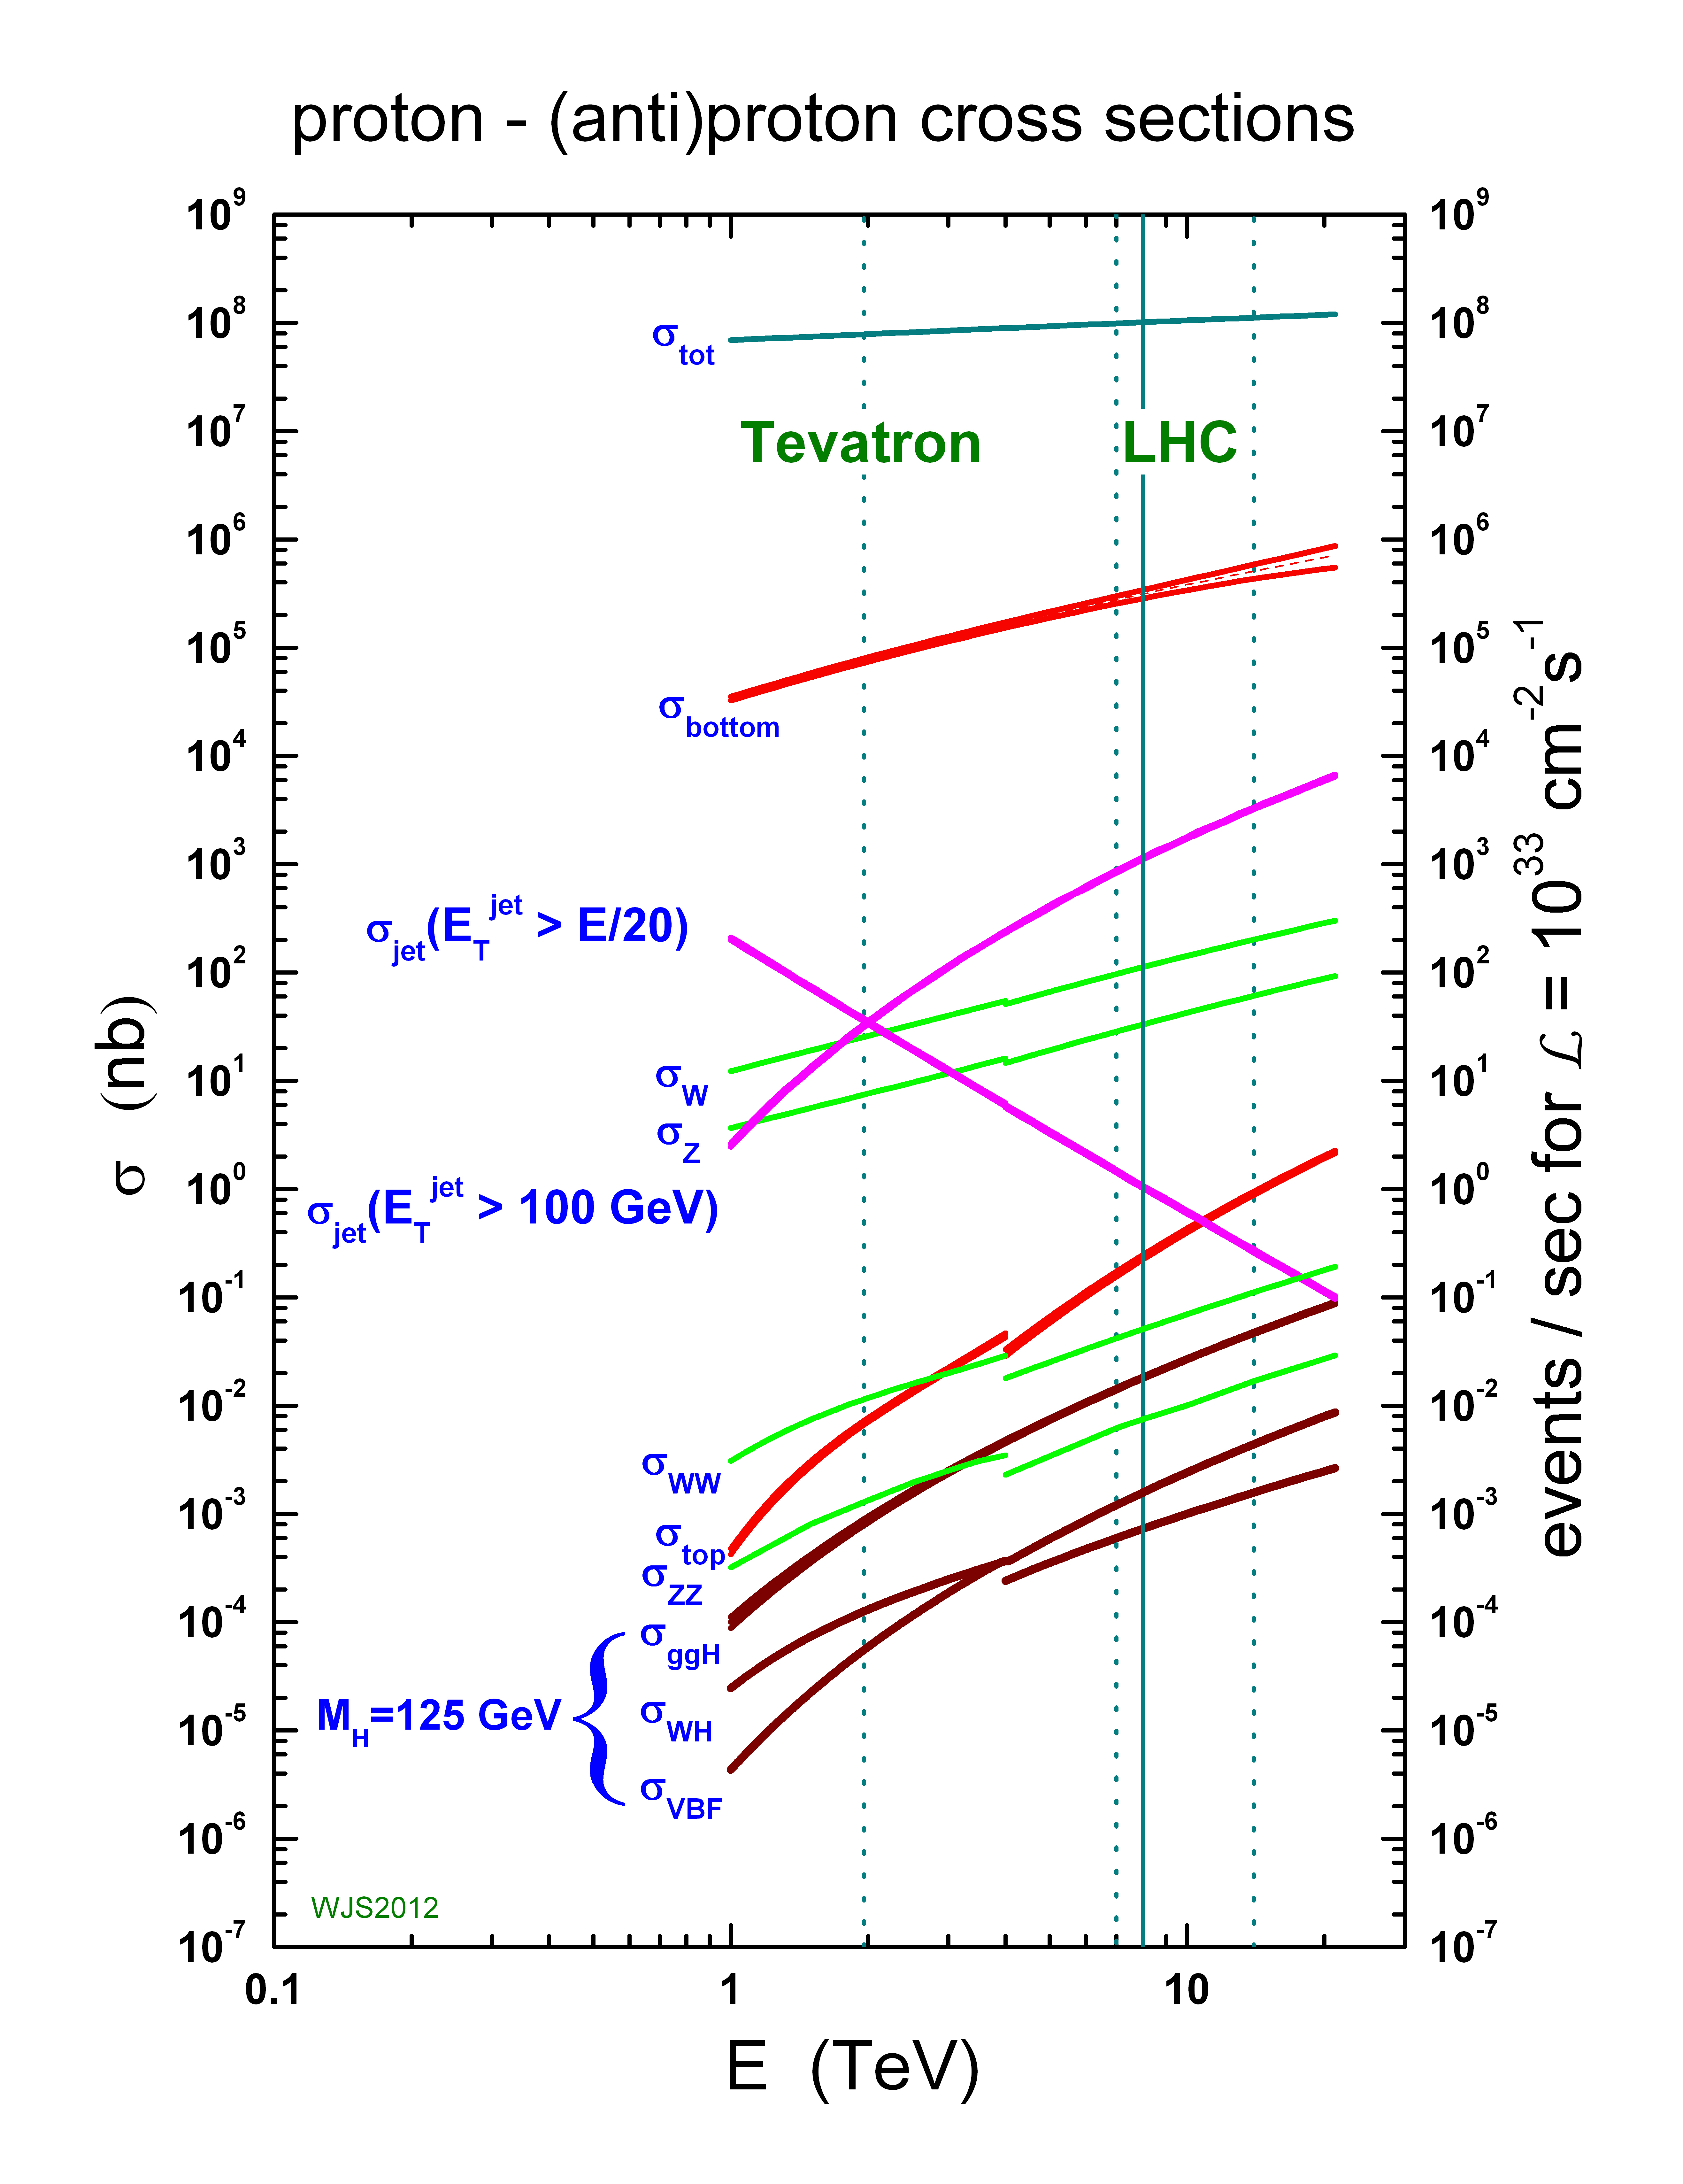
\includegraphics[width=.7\textwidth]{figures/lhc_decay_modes.jpg}
    \caption{Production Cross Sections for the LHC}
    \label{fig:lhc_decay_modes}
  \end{figure}

  Point out that there is very low chance for double scattering or two interesting interactions in one bunch crossing. Point out cross section of Z boson, point out the NJets rule.

\section{The CMS Detector}
  \subsection{The Inner Tracker}
  \subsection{The Electromagnetic Calorimeter} \label{sec:ECAL}
    Need to put in the deadzone here.
  \subsection{The Hadronic Calorimeter}
  \subsection{The Muon System}
  \subsection{Fiducial Area} \label{sec:fiducial_area}
    the wierd eta deadzone, very forward stuff.
  \subsection{Event Triggering} \label{sec:event_triggering}
    trigger turn ons, list the triggers we use, Level 1 and HLTs?


\section{Physics Objects}
  \subsection{Particle flow and jet clustering} \label{sec:particle_flow}
  \subsection{Vertex Selection}
    \todo{Rewrite: We require the presence of at least one primary vertex satisfying the standard quality criteria; 176 namely,vertexisnotfake,ndf>4,ρ<2cm,and|z|<24cm.}
  \subsection{Electron Measurement Pipeline} \label{sec:electron_measurement_pipeline}
    Tracker, ecal, distinguishing between electrons and muons. Cite the CMS paper on electron energy reco..
  \subsection{Muon Measurement Pipeline} \label{sec:muon_measurement_pipeline}
    Tracker muons, global muons, muon system
  \subsection{Photon Measurement Pipeline}
    ECAL measurements, lepton conversions.
  \subsection{Jets} \label{sec:jets}
    Describe charged hadron subtraction, JECs ~\cite{JERC}
    pfCHSjets with L1FastL2L3 corrections (MC), L1FastL2L3L2L3residual corrections (data).
    \verb=Summer16_23Sep2016V3= JEC payload used to correct jets
    Need to put in blurbs about L1 Pile Up Corrections, L2L3 MC-Truth Corrections, and L2L3Residual Corrections (data only). Short descriptions here: https://twiki.cern.ch/twiki/bin/view/CMS/IntroToJEC
    pfjetID


    Good info in Vince's Thesis and here: https://arxiv.org/pdf/1607.03663.pdf
    Roughly: L1 -- (pileup offset correction) pileup correction use QCD MC to get avg energy change to jet with and without pileup overlay. Look in 2D plane of $\eta$ and \pt, get correction.
    L2L3 -- (simulated responce correction) Look at dijet events in MC, see how energy reco is different across \pt and $\eta$, correct for it.
    L2L3 Residual -- (Residual Corrections for data) Make MET 0 in dijet/ZJet/GammaJet events.
  \subsection{B-Tagging} \label{sec:b-tagging}

  \subsection{MET Reconstruction} \label{sec:MET_reco}
    Make sure to add bits about sources of MET and the Type 1 correction
  \subsection{MET Filters} \label{sec:met_filters} 
    We apply certain filters that kill events, these are called MET filters but include things like beam halo as well.

\section{Monte Carlo}
  \subsection{SUSY Simulation} \label{sec:susy_simulation}

\section{Datasets} \label{sec:datasets}
We use dilepton trigger events, as will be described in section \ref{sec:leptonic_final_states}